\documentclass[aspectratio=169]{beamer}
\usetheme{metropolis}

\usepackage[utf8]{inputenc}
\usepackage[OT4]{polski}
\usepackage{flexisym}
\usepackage{parskip}
\usepackage{algpseudocode,amsmath}
\newcommand{\var}{\texttt}
\newcommand{\assign}{\leftarrow}
\usepackage{listings}
\usepackage{color}
\usepackage{capt-of}

\definecolor{dkgreen}{rgb}{0,0.6,0}
\definecolor{gray}{rgb}{0.5,0.5,0.5}
\definecolor{mauve}{rgb}{0.58,0,0.82}

\lstset{frame=tb,
	language=c++,
	aboveskip=3mm,
	belowskip=3mm,
	showstringspaces=false,
	columns=flexible,
	basicstyle={\small\ttfamily},
	numbers=none,
	numberstyle=\tiny\color{gray},
	keywordstyle=\color{blue},
	commentstyle=\color{dkgreen},
	stringstyle=\color{mauve},
	breaklines=true,
	breakatwhitespace=true,
	tabsize=3
}


\title{Zadanie 10. Podział liczby}
\subtitle{Adrian Rupala}

\begin{document}
	\frame {
		\titlepage
	}

	\frame {
		\frametitle{Treść zadania}
		\fontsize{10pt}{7.2}\selectfont
		Liczbę naturalną $C$ można przedstawić jako sumę parami różnych liczb naturalnych. \\Na przykład jeśli $C = 6$, to możemy C przedstawić na cztery sposoby:
		\\$1+2+3$
		\\$1+5$
		\\$2+4$
		\\$6$ 
		\\a jeśli $C = 10$, to takimi podziałami są:
		\\$1+2+3+4$
		\\$1+2+7$
		\\$1+3+6$
		\\$1+4+5$
		\\$1+9$
		\\$2+3+5$
		\\$2+8$
		\\$3+7$
		\\$4+6$
		\\$10$
		\\Skonstruuj algorytm wyczerpujący z nawrotami, generujący wszystkie podziały podanej liczby naturalnej $C$.~
	}

	\frame{
		\frametitle{Definicje}
		\fontsize{14pt}{7.2}\selectfont
		\large Algorytm z nawrotami to algorytm wyszukiwania wszystkich lub kilku rozwiązań. Polega on na znajdowaniu wyniku metodą „prób i błędów”, wszelako z~oznaczeniem niepowodzeń, dzięki czemu te same błędy nie są popełniane dwukrotnie.~
		
		\large Jeżeli problem pozwala na zastosowanie algorytmu wyszukiwania z nawrotami, to metoda ta może być znaczenie efektywniejsza niż wyszukiwanie wyczerpujące (zakładające przeszukiwanie wszystkich rozwiązań), ponieważ pojedynczy test może wyeliminować nie jedno, a wiele rozwiązań niedopuszczalnych.~
			
	}

	\frame{
	\frametitle{Definicje}
	\fontsize{14pt}{7.2}\selectfont
	\large Rekurencja to technika programowania, dzięki której funkcja, procedura lub podprogram jest w stanie w swoim ciele wywołać samą siebie. Pozwala ona łatwo wykonać wiele zadań, w których zachodzi potrzeba obliczenia wyników cząstkowych do obliczenia całości. ~
		
	}

	\begin{frame}[fragile]
	\frametitle{Rozwiązanie - kod C++}
	
	\begin{lstlisting}[basicstyle=\footnotesize]
	void podzial(int C, int obecny, int* tablica, int index) {
		if (obecny + tablica[index] == C) {
			for (int i=0; i <= index; i++) {
				cout << tablica[i] << " ";
			}
			cout << endl;       
			;
		} else if (obecny + tablica[index] > C) {
			;
		} else {
			for(int i = tablica[index]+1; i < C; i++) {
				tablica[index+1] = i;
				podzial(C, obecny + tablica[index], tablica, index+1);
			}
		}
	}
	\end{lstlisting}
	
	\end{frame}

	\begin{frame}[fragile]
	\frametitle{Rozwiązanie - kod C++}

			\begin{lstlisting}[basicstyle=\footnotesize]
	int main(){   
		int C = 0;
	
		cout << "Podaj liczbe: " << endl;
		cin >> C;
		cin.get();
		cout << "======" << endl;
	
		for(int i = 1; i < C; i++) {
			tablica[0] = i;
			podzial(C, 0, tablica, 0);
		}
	
		cin.get();
		return 0;
	}
			\end{lstlisting}

	
	\end{frame}

	\begin{frame}[fragile]
	\frametitle{Wykonanie kodu}
		\begin{columns}
			\column{.5\textwidth}
			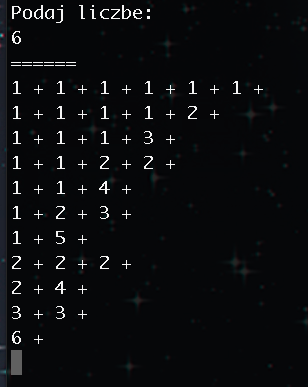
\includegraphics[width=.6\linewidth]{source/1.png}
			\captionof{figure}{Wynik dla liczby 6.}
			
			\column{.5\textwidth}
			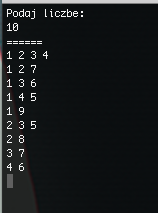
\includegraphics[width=.6\linewidth]{source/2.png}
  			\captionof{figure}{Wynik dla liczby 10.}

		\end{columns}
	\end{frame}

	
		
	\frame{
		\centering \Huge
		\emph{Dziękuję za uwagę!}
	}
	
\end{document}
